\subsection{Zpracování elektrické srdeční aktivity}
\label{subsec:zpracovani_ekg}
Pro zpracování EKG záznamů byla implementována metoda podle Kalidase a
Tamila~\cite{kalidas2017}, která je založena na stacionární vlnkové transformaci
(\gls{SWT}). Metoda vychází z populárního Pan-Tompkinsova~\cite{Tompkins1985}
algoritmu ale pro odstranění šumu a zvýraznění QRS komplexů používá \gls{SWT}
namísto pásmové propusti. Stacionární vlnková transformace je metoda rozkladu
signálu na jednotlivá frekvenční pásma pomocí mateřské vlnky~\cite{Nason1995}.

\begin{figure}[H]
    \begin{center}
        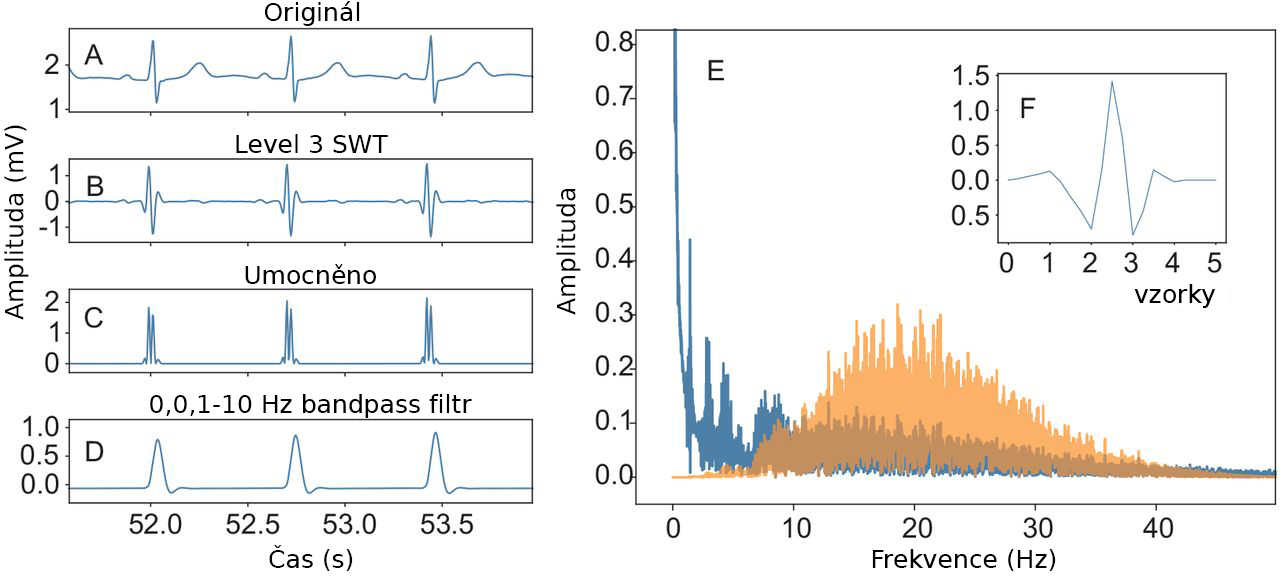
\includegraphics[width=1\linewidth]{figures/kalidas2017}
        \caption{\textbf{A-D)} Kroky zpracování EKG pro algoritmus podle
            Kalidase a Tamila~\cite{kalidas2017} \textbf{E)} Frekvenční spektrum
            nefiltrovaného EKG se vzorkovací frekvencí 250~\si\Hz~(modrá) a EKG po
            SWT 3. řádu (oranžová). \textbf{F)} vlnka rodiny Daubechies 3. řádu.
            (Upraveno a převzato z~\cite{Porr2019})}
        \label{fig:kalidas_processing}
    \end{center}
\end{figure}

V tomto algoritmu se stacionární vlnková transformace provádí na EKG signálu
využitím Daubechiesové vlnky třetího řádu. Po provedení \gls{SWT} se extrahují
koeficienty, které se následně vyčíslí na čtverec. Následně je využito filtrace
pásmovou propustí ke zvýšení citlivosti a přesnosti detekce. Postup detekce R
vln na filtrovaném signálu je pak totožná s detekcí Pan-Tompkinsova
algoritmu~\cite{Tompkins1985}. Jednotlivé částí zpracování lze vidět na
Obr.~\ref{fig:kalidas_processing}.

\subsubsection{Metodika výběru QRS detektoru}
\label{subsubsec:vyberqrs}
Vzhledem k tomu, že neexistuje žádný jednotný standard či systematický postup
pro zpracování EKG a výběr \enquote{správného} QRS detektoru pro určitou
aplikaci, tak bylo v rámci této práce realizováno statistické porovnání
populárních algoritmů. Jakožto měřítko přesnosti QRS detekce algoritmu bylo
vycházeno z výpočtu absolutní vzdálenosti od původní \enquote{skutečné} polohy R
vlny. Pro benchmarking detektorů byly tedy použity následující anotované
datasety:

\begin{table}[h]
    % \footnotesize
    \begin{center}
        \caption{\label{tab:bench_datasets} Vybrané datasety pro benchmarking
            QRS detektorů z PhysioNetu~\cite{PhysioNet}}
        \renewcommand{\arraystretch}{1.3}
        \begin{tabular}{p{12cm}c}
            \toprule
            \textbf{Dataset}                                                                                                 & \textbf{Probandi} \\ \midrule
            MIT-BIH Arrhythmia Database~\cite{MITBIHArrhythmia}                                                              & 48                \\
            MIT-BIH Normal Sinus Rhythm Database~\cite{Beth1990}                                                             & 18                \\
            Glasgow University Database~\cite{GUDB}                                                                          & 25                \\
            Fantasia Database~\cite{FANTASIA}                                                                                & 40                \\
            Lobachevsky University Electrocardiography Database~\cite{LUDB}                                                  & 200               \\
            Simultaneous physiological measurements with five devices at different cognitive and physical loads~\cite{IFADO} & 13                \\
            Pulse Transit Time PPG Dataset~\cite{USYD}                                                                       & 22                \\
            \bottomrule
        \end{tabular}
    \end{center}
\end{table}

Byly vybrány různorodé datasety za účelem zjištění adaptability algoritmu. Pro
statistické zpracování bylo využito lineárních smíšených modelů (\gls{LMM}). Použité
statistické metody jsou podrobněji popsány v kapitole~\ref{sec:statisticke_metody}.
Pro srovnání metod byl v programovacím jazyce R vytvořen následující statistický model:
\begin{equation}
    \text{Skore} = \beta_0 + \beta_1\text{Metoda} + u_{\text{Dataset}} + u_{\text{Participant}} + \epsilon
\end{equation}
který specifikuje lineární smíšený model pomocí funkce \texttt{lmer} z balíku
\texttt{lme4}\footnote{\url{https://github.com/lme4/lme4}}. Model byl použit k
predikci závislé proměnné Skore na fixním efektu $Metoda$ a dvou náhodných
efektech: $Dataset$ a $Participant$. Dále problematice této sekce není věnována
pozornost, jelikož není předmětem této práce. 

\subsection{Zpracování respirační aktivity}
\label{subsec:zpracovani_rsp}
Pro zpracování respirační aktivity byl implementován
algoritmus~\cite{Khodadad2018}, který je založen na průchodech nulou (\gls{ZC},
Zero-Crossing). Originální signál je nejdříve filtrován pásmovou propustí pro
odstranění stejnosměrné složky, aby bylo možné spolehlivě detekovat \gls{ZC}. K
tomu byla využita pásmová propust 0,05--3~Hz , která zároveň zachovává dechové
frekvence menší než tři a vyšší než 180 dechů za minutu. Následně jsou pomocí
logických operací detekovány indexy náběžných a sestupných průchodů nulou, mezi
kterými došlo k hledání lokálních extrémů.

\begin{figure}[h]
    \begin{center}
        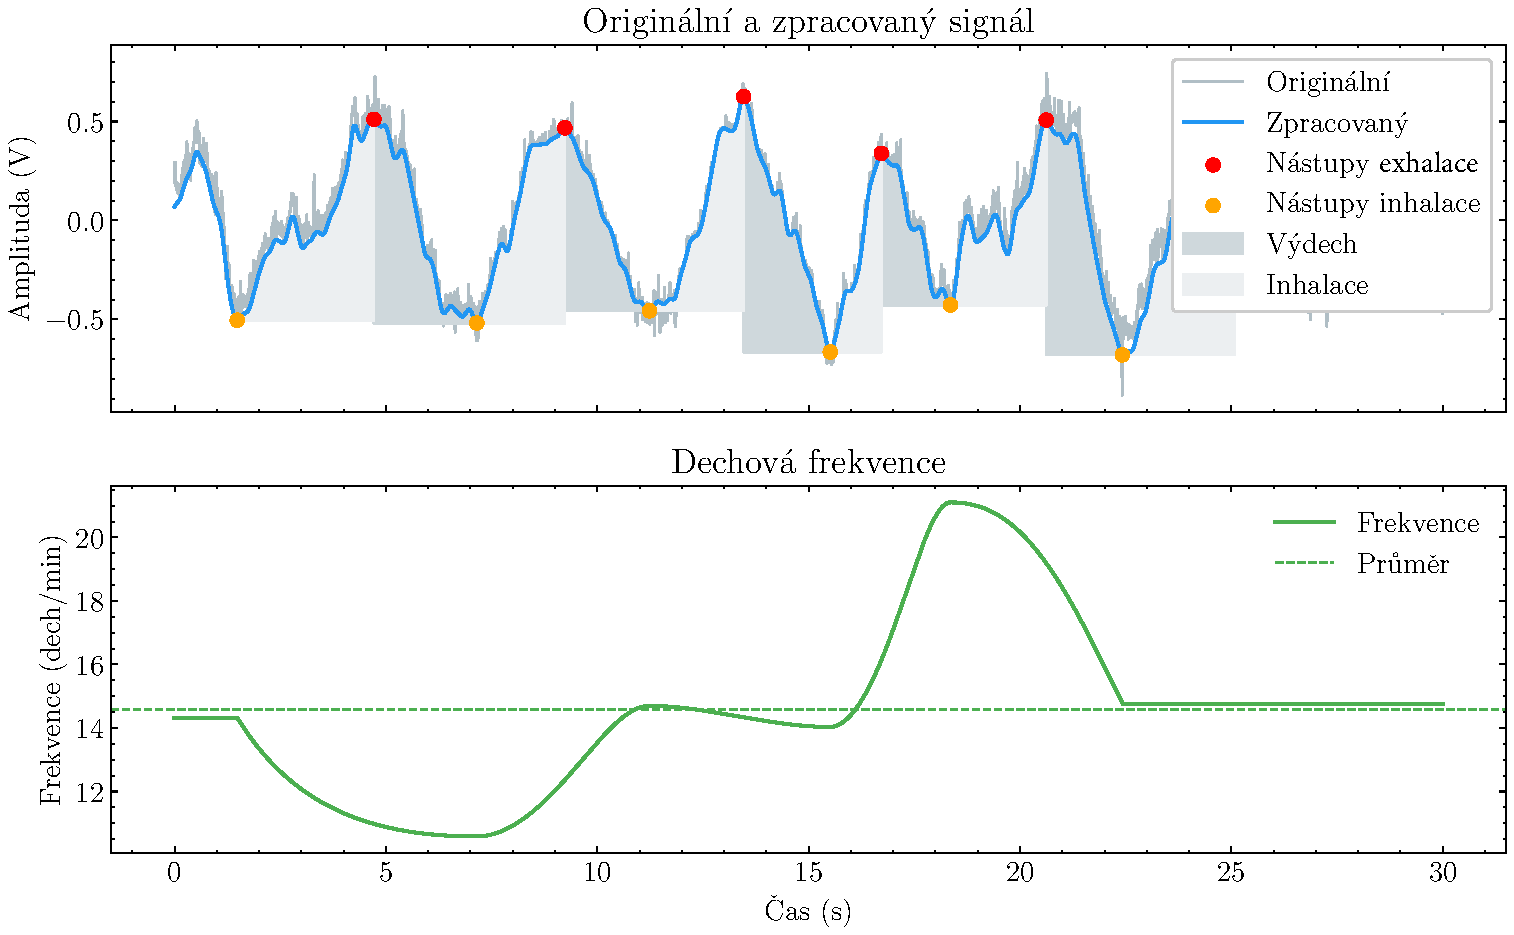
\includegraphics[width=1\linewidth]{figures/rsp_test}
        \caption{Příklad zpracování RSP pomocí implementované metody}
        \label{fig:rsp_test}
    \end{center}
\end{figure}

Zachovány jsou ve výsledku pouze ty extrémy, které mají minimální vertikální
vzdálenost od svého přímého souseda, tudíž kritérium pro detekci odlehlých
hodnot bylo definováno v absolutním rozdílu amplitud mezi sousedními extrémy.
Aplikace metody na reálném signálu lze vidět na Obrázku~\ref{fig:rsp_test}.

\subsection{Zpracování elektrodermální aktivity}
\label{subsec:zpracovani_eda}
Zpracování elektrodermální aktivity vychází z metod~\cite{vanhalem2020}
a~\cite{posada2016}. Signál je nejdříve filtrován Butterworthovou horní propustí
4. řádu s mezní frekvencí 3~\si\Hz. Následně je ze signálu extrahována fázická a
tonická složka pomocí dolní a horní propusti o mezních frekvencích 0,05~\si\Hz.

\begin{figure}[h]
    \begin{center}
        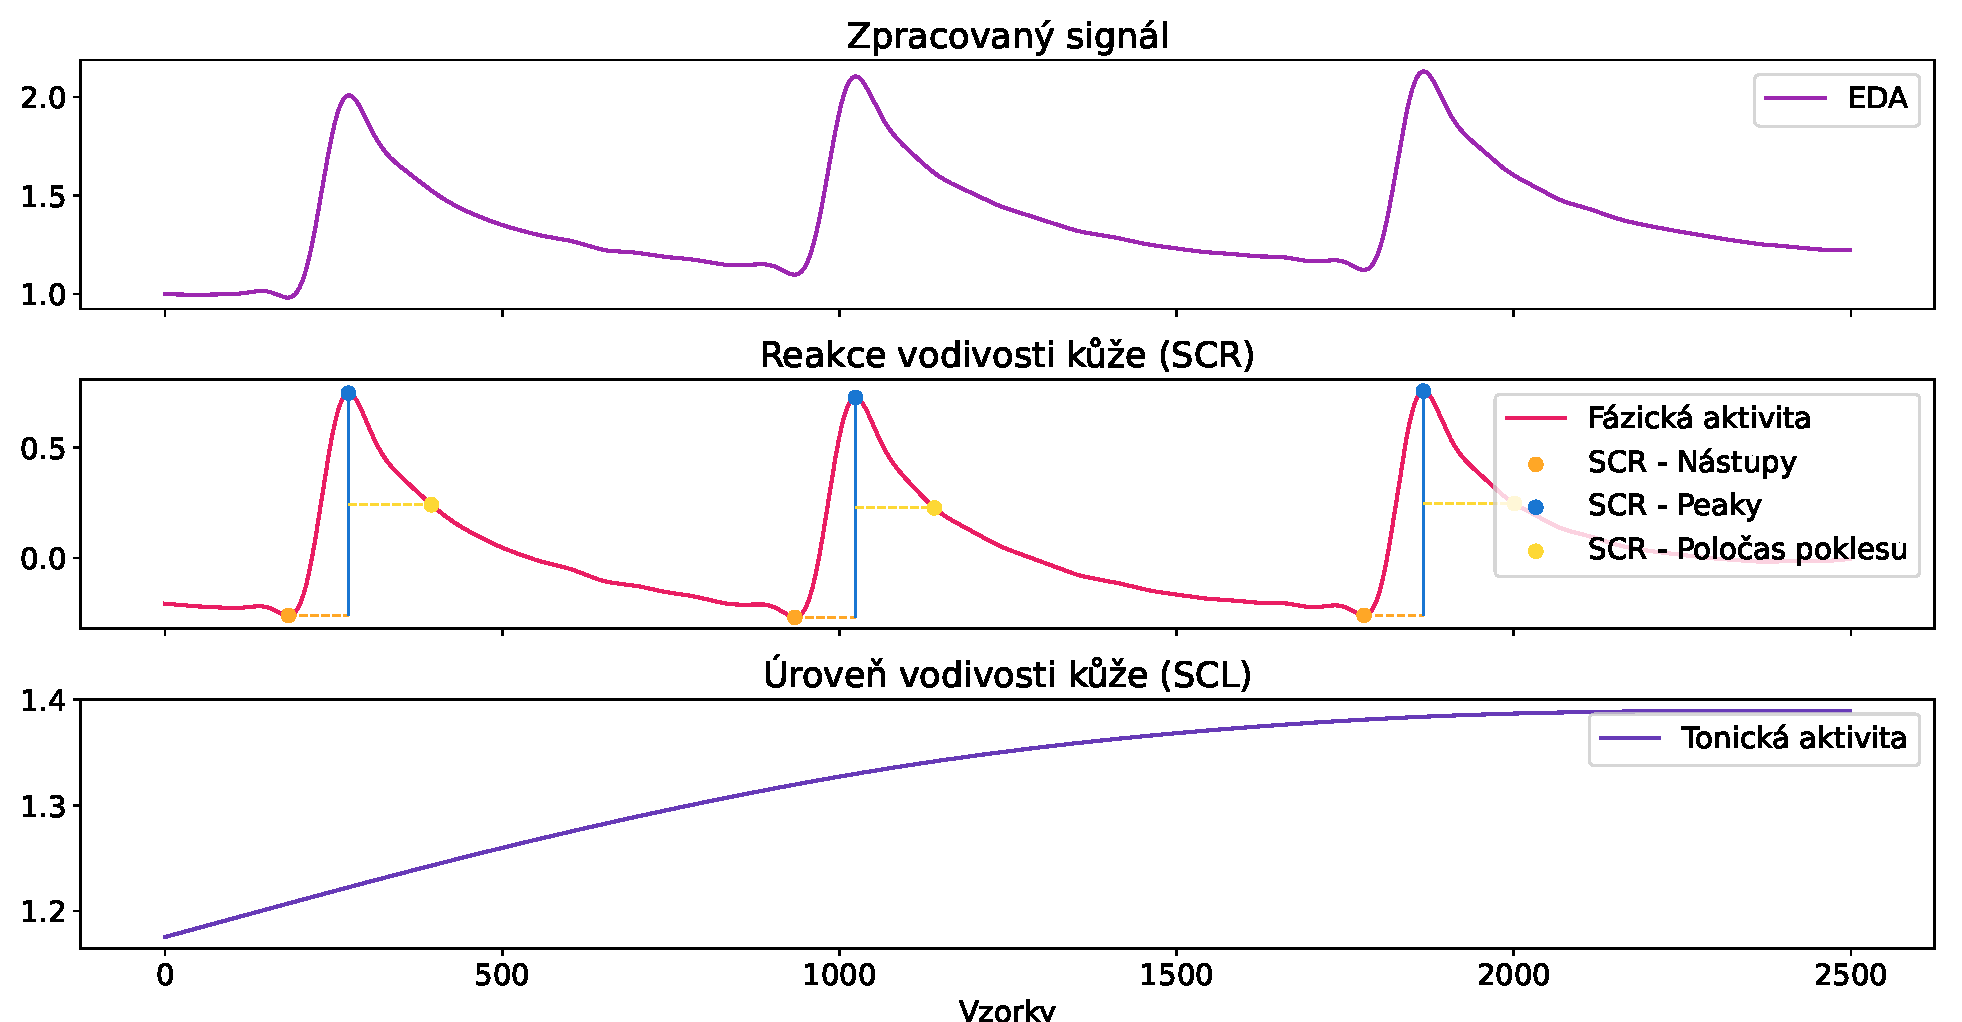
\includegraphics[width=1\linewidth]{figures/eda_test}
        \caption{Příklad zpracování EDA pomocí implementovaných metod}
        \label{fig:eda_test}
    \end{center}
\end{figure}

Dále byl použit Savitzky-Golayův frekvenčně neselektivní filtr k dalšímu
vyhlazení fázické složky za účelem hledání \gls{SCR} vrcholků. K detekti
vrcholků byla využita funkce \texttt{find\_peaks()} z knihovny
Scipy\footnote{https://docs.scipy.org}. Kritérium pro detekci vrcholků bylo
definováno jako konzistentní nárůst o 0,5s následovaný stejným poklesem.
Výsledek aplikované metody lze vidět na Obrázku~\ref{fig:eda_test}.

\subsection{Neurokit}
\label{subsec:neurokit}
Knihovna \textit{Neurokit2}\footnote{\url{https://neuropsychology.github.io/NeuroKit}},
na jejíž vývoji se podílím, poskytuje pokročilé metody pro zpracování a
vizualizaci biosignálu. Jednotlivé metody zároveň nabízejí možnost si vybrat z
mnoha implementovaných algoritmů. V této práci byla knihovna použita pro
zpracování respirační, elektrodermální a elektrické srdeční aktivity včetně
zpracování a výpočet \gls{HRV} parametrů.
